\chapter{Heritage of ice reservoirs}

\cleanchapterquote{Before the artificial glacier, we struggled to get any barley. But now we can grow many
  crops, even potatoes, which need to be planted earlier in the spring, but sell for much more money.
}{Tashi Tundup}{(A 76 year old farmer in Ladakh)}

This chapter provides conclusions based on research findings from data collected on AIRs in Switzerland and India,
as well as discussion and recommendations for future research. This Chapter will review the purpose of the
study, research questions, literature review, and findings of the study. It will then present conclusions,
discussion of the conclusions, and recommendations for practice and for further research.

\section{Summary}

Cryosphere fed irrigation networks are completely dependant on the timely availability of meltwater from
glaciers, snow and permafrost. With the accelerated decline of glaciers, these irrigation networks can no longer
deliver adequate water to sustain agricultural output and take advantage of the complete growing season. As a
consequence, some mountain villages have either been abandoned or lie on the brink of desertification
\cite{grossmanHimalayanGlaciersMelt2015}.

In the past few decades, artificial ice reservoir (AIR) technologies have provided much needed relief to these
water-stressed communities. These strategies revolve around augmenting their glacial ice reservoirs with
man-made ones that provide supplementary irrigation during the spring. In the context of the observed present
and predicted global glacier shrinkage, the development of such water storage technologies is crucial to ensure
continued sustenance of cryosphere-fed irrigation networks.

AIR observations and investigations date back to the mid-2000s \cite{tveitenGlacierGrowingLocal2007}. The vast
majority have been published in the 2010s, mostly using qualitative methods. However, quantifications of their
storage capacity differ widely amongst these publications. \citep{baglaArtificialGlaciersHelp1998,
norphelSnowWaterHarvesting2015, nusserSociohydrologyArtificialGlaciers2019}. Because small-scale processes,
complex feedbacks and non-linearities govern their evolution, modelling the volume evolution of ice stupas is
only feasible if backed up with comprehensive input, calibration and validation datasets.

In response, we conducted measurement campaigns using drones, flowmeters and weather stations on almost a dozen
AIRs across two locations (India and Switzerland), over four winters (2019, 2020, 2021 and 2022) and using two
different construction methods (traditional and automated). Each dataset contained information on the
meteorological conditions, fountain characteristics and AIR volume evolution. 

The primary objective of this thesis was to improve our understanding about the response of AIRs to changes in
their construction location. The secondary objective was to propose automated constuction strategies that reduce
water losses and maintenance efforts.  

\section{Conclusions}

\begin{figure}[htb]
	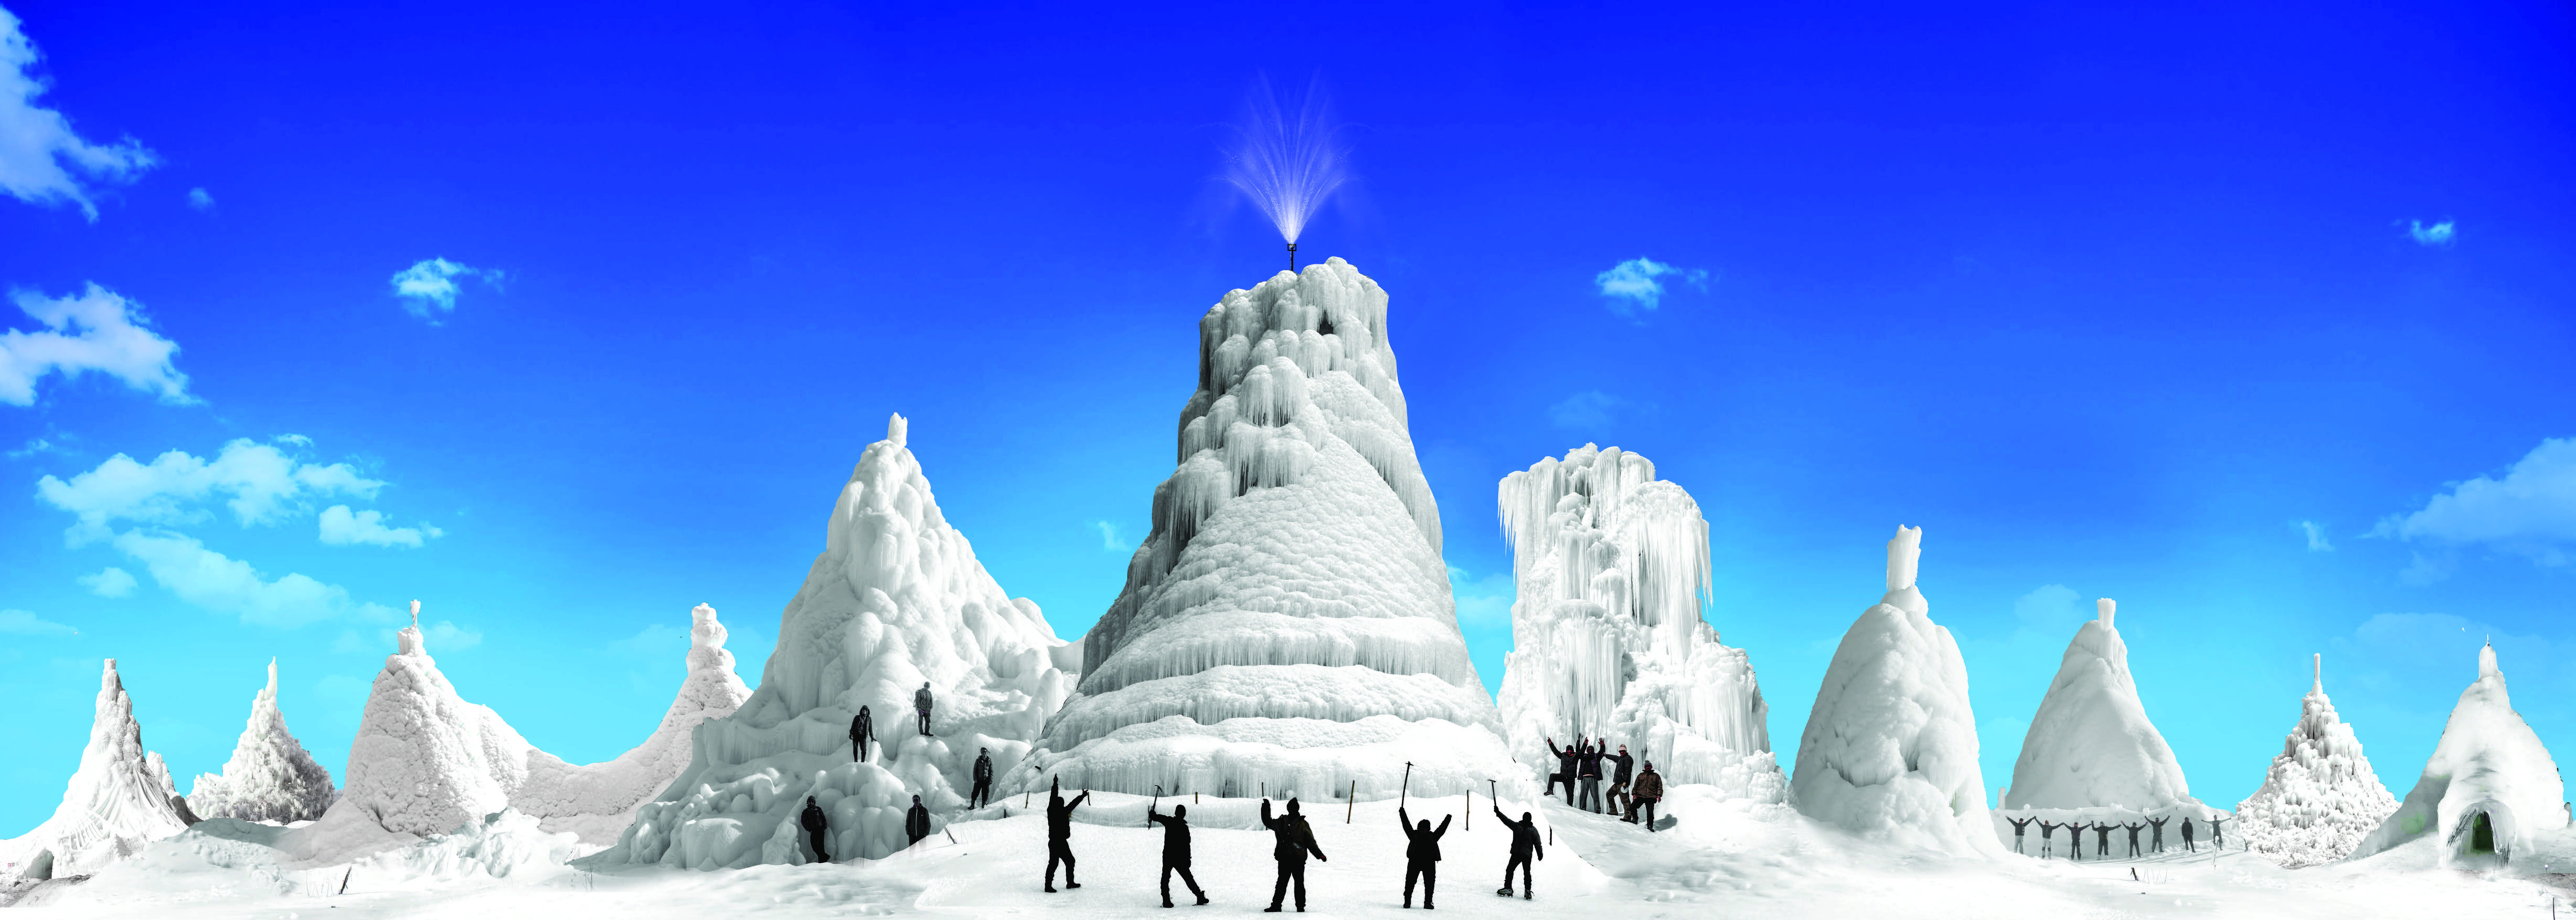
\includegraphics[width=\textwidth]{figs/AIRs_Ladakh}
	\caption{Compilation of AIRs built in different villages of Ladakh.}
	\label{fig:airs_ladakh}
\end{figure}

In paper I, an AIR model was designed to resolve surface processes and used to compare their volume evolution
in Indian Himalayas and the Swiss Alps. In paper II, the evolution of AIRs using different fountain
scheduling strategies were compared. In paper III, the possibility of sustaining artificial ice reservoirs
perpetually was explored. The results of these papers can be summarised as follows:

\begin{enumerate} 

\item Volumes of ice stupas located in different regions may differ by an order of magnitude. The differences
  could be attributed to the accelerated sublimation process in colder and drier regions.

\item Water losses of ice stupas may be upto 80 \% due to excessive water input. However, water supply
  management through fountain scheduling strategies can produce icestupas of similar volumes while reducing upto
  one-tenth of their water supply.

\item Traditional construction systems demand significant maintenance efforts since they are prone to freezing
  events in the fountain pipeline. However, automated construction systems can prevent these events to make the
  construction process maintenance-free.

\item There exist locations with favourable weather conditions and sufficient water supply that can sustain
  artificial ice reservoirs perpetually.

\end{enumerate}

\section{Discussion}

\subsection{The state of ice stupa technology}

The thesis shows one strategy that can improve the water-use efficiency of AIRs. We chose this strategy
because it enables the use of the AIR model in a simple and effective manner. Ice stupa construction can
significantly be improved with sufficient engineering expertise. The fountain nozzle design is crucial for
increasing the ice volume obtained. However, no methodology currently exists to rank the several fountain
nozzles used for construction. An ideal pipeline configuration could make this technology cheaper and
maintenance free. However, optimization of the pipeline material and diameters is yet to be performed---despite
the time lost on pipeline freezing events and the potential cost reduction with cheaper pipeline materials and
sizes. Therefore, we strongly encourage the engineering community to get involved and push the limits of the
cost-effectiveness, size, and survival duration of artificial ice reservoirs. 

\subsection{Feasibility of constructing artificial glaciers}

By definition, all glaciers, including the smallest ones, are bodies of sedimentary ice which were built up by
progressive snow compaction and firnification and flow downhill under the influence of gravity
\cite{benndouglasiGlaciersGlaciation2014}. Hence, because of their genesis and composition, AIRs differ from
glaciers. But when classified in terms of size and survival duration, AIRs exhibit similar characterestics to
very small glaciers. The glossary of glacier mass balance and related terms by
\citet{cogleyGlossaryGlacierMass2010} defines very small glaciers or glacierets as follows:

\begin{thesis_quotation}
  A very small glacier, typically less than 0.25 $km^2$ in extent, with no marked flow pattern
  visible at the surface. To qualify as a glacieret, an ice body must persist for at least two consecutive
  years. Glacierets can be of any shape, and usually occupy sheltered parts of the landscape. Windborne snow and
  avalanches can be dominant contributors to the accumulation of glacierets. 
\end{thesis_quotation}

This rather broad definition of glacierets or very small glaciers may be the one best suited for AIRs. Based on
this definition, we can define "artificial glaciers" as ice bodies that are both larger in area and last longer
than two consecutive years. Manmade ice structures can, in theory, occupy any area provided for their
construction. But can AIRs, like glaciers, also survive the summer and compound their size every consecutive
winter? 

We believe so, mainly because AIRs built in certain favourable locations have been measured with areas upto 0.15
$km^2$ \cite{nusserSociohydrologyArtificialGlaciers2019} and observed to last for two consecutive years. These
feats were achieved with rudimentary tools available to local farmers and almost no water supply management.
Therefore, with the automated construction strategy developed in this thesis, AIRs can achieve areas and
survival durations that warrants their classification as artificial glaciers.

% Two ways to improve size and duration of AIRs

\section{Future research direction}

Insights from this research could contribute to efforts to better estimate the future potential of AIRs for
climate change adaptation and mitigation under multiple plausible future climatic, demographic, economic, and
land use scenarios. Finally, the scripts developed are also shared and could be adapted in various contexts to
efficiently calculate ice surface processes over arbitrary complex and/or large geometries, including in
non-mountain applications; a further benefit of the “Open Science” approach taken.

\subsection{Quantification and development of ice terraces}

Although this thesis focuses on ice stupas, their ice volumes pale in comparison with ice terraces
\citep{nusserSociohydrologyArtificialGlaciers2019}. This is because ice stupas are limited by their fountain's
spray radius and its maximum height. However, ice terraces have no such limitations. Their thickness is only
limited by the water supply rate or weather conditions and they can occupy any construction area provided. But
despite this, ice stupas are the preferred method of ice harvesting due to their longer survival duration and
reduced construction effort.

Implementing automated construction strategies for ice terraces could help change this. Such a construction
strategy can compound their size every consecutive winter and turn them into artificial glaciers with minimal
maintenance requirements. Therefore, future research direction should aim to answer the following questions:

\begin{itemize}

  \item How can ice terrace construction systems be engineered to reduce their water losses and maintenance
    efforts?
  \item Where can ice terraces form artificial glaciers ? 

\end{itemize}

The methodology developed in this thesis can be used for such an analysis. 

\subsection{Model development}

\subsubsection{Towards accuracy}


\subsubsection{Towards predictions}

There is still a substantial potential for developing better models to calculate AIR volumes. Modelling the
future is fundamentally different from simulating the past: In the past the model serves as a tool for
interpreting and best exploiting field measurements - and can be directly constrained by these. Models for the
future must understand climate variability to be able to yield realistic projections. Almost all methodological
steps in the modelling of future AIR runoff are subject to possible enhancements, always bearing in mind that we
will only know whether the effort led to an enhanced or even a worsened performance, when we're old... 

\subsection{Development of AIR suitability metrics}


\section{Final thoughts}

Progressing glacier melt and the associated growing number of lakes rises the threat of glacier lake outburst
floods (GLOFs); at the same time declining melt water supply changes the hydological regime, resulting in
changing water availability especially during dry seasons. AIRs could become a crucial water resource management
strategy to deal with both these high and low flow water hazards.


% In a first step, a measurement
% campaign will be conducted on existing ice terrace construction locations using weather stations, discharge
% loggers and drones to acquire calibration and validation datasets to develop an ice terrace model. In a second
% step, a construction campaign will be conducted using an automation hardware designed to implement water supply
% management using the ice terrace software. In a third step, possibility of creating artificial glaciers using
% glacial lakes will be explored through simulations and later validated through construction campaigns.

% Successfully creating such an artificial glacier could provide unprecedented scientific insights in the
% processes governing glacial formation. More importantly, they could be used to harvest glacial lakes into ice
% reservoirs and pave the way for scalable climate adaptation strategies.

% \subsubsection{Educational tool}

% , climate change communication, scientific experiments

% \subsubsection{Sustainable tourism}

% Sculpture, religious monument, accomodation, ice climbing

% With a special focus on ice stupas, a mass and energy balance model was developed and used as a tool to quantify
% the influence of meteorological conditions and fountain characteristics. The meteorological and fountain
% observations were used as model input; AIR volume observations were used to calibrate the model parameters and
% validate its ice volume estimations.

% The model has been shown to perform excellently when calibrated with the AIR datasets.  It could be shown that
% the maximum volume of AIRs located in the IN and CH regions differ by an order of magnitude. These differences
% were caused by the stronger sublimation process due to the colder and drier weather conditions of the IN region. 

% AIR maintenance requirement was reduced and their fountain freezing events were prevented by developing an
% automated construction strategy. Fountain operation was made 8 times more efficient and effortless through the
% use of an automation system that scheduled discharge rates based on the recommendations of the AIR model. 

% \begin{itemize} 

% \item[\tiny{$\blacksquare$}] Colder, drier and less cloudy construction locations form long-lasting AIRs with
%   higher maximum ice volumes. 

% \item[\tiny{$\blacksquare$}] Weather-sensitive fountain systems produce larger and efficient AIRs effortlessly. 

% \end{itemize}

% There is no, and probably will never be, consensus about how to define AIRs. Therefore, no conclusive definition
% of AIRs is promoted in this thesis, either.
% The rise of ice harvesting technologies has pushed the boundaries of the size and survival duration of manmade
% ice structures.

% \begin{itemize} 

% \item Identification of favourable locations using AIR suitability and water scarcity index.

% \item Cosistupa model development for inspecting ice surface processes.

% \end{itemize}

% \subsection{Ice stupas vs Ice terraces}

% \begin{table}[htb]
% 	\begin{tabularx}{\textwidth}{X | X | X | X}
% 		\hline
%     \textbf{Technology}& \textbf{Water storage}& \textbf{Daily meltwater supply (days)}& \textbf{Duration} \\
%     \hline
% 		Ice terraces			& < 30				     & 2 months				\\
%     Ice stupas        & < 10             & 5				\\
% 		\hline
% 	\end{tabularx}
% 	\label{tab:table1}
% 	\caption{This is a caption text.}
% \end{table}
